\begin{tcolorbox}[colback=backblue]
\textbf{Example:} We can see a use of the likelihood ratio in a \emph{classification} problem. Suppose we record the quantity $\theta\in[0,\pi]$ in particle collisions of the type $e^{+}e^{-}\rightarrow \mu^{+}\mu^{-}$, where $\theta$ is the angle shown in Figure~\ref{fig:eemm}. The distribution of $x=\cos(\theta)$ will be symmetric around 0 if the exchange is mediated by a photon and the cross-section will be proportional to $1+x^{2}$ . Instead, the contribution of the $Z$ boson means that  the distribution will be proportional to $a(1+x^{2})+bx$, where $a$ and $b$ are proportional to the vector and axial-vector couplings.  We define $H_1$ as the latter (scattering via a $Z$ boson)  and $H_0$ as the former (scattering via a $\gamma$) hypotheses. For each event we record, we can calculate $\Lambda$ as, 
\begin{eqnarray}
   \Lambda & = & \dfrac{f(x|H_1)}{f(x|H_0)}.
\end{eqnarray}
where the normalised p.d.fs are, 
\begin{eqnarray}
   f(x|H_1) & \propto & a(1+x^{2})+bx \\
   f(x|H_0) & \propto & 1+x^{2} 
\end{eqnarray}
We can use the \textsf{rv\_continuous} class from the \textsf{scipy.stats} module to define our probability density functions  
\begin{lstlisting}[style = Python]
import numpy
from scipy import stats
import matplotlib.pyplot as plt
plt.rcParams.update({'font.size': 14})

# x = cos(theta)
# pure photon exchange ~ 1+x^2
class photon_exchange(stats.rv_continuous):
  def _pdf(self,x) :
    N = 8./3
    return (1+x*x)/N
  def _get_support(self):
    return -1,1

# Z* exchange ~ 1+x^2
class Z_exchange(stats.rv_continuous):
  def _pdf(self,x) :
    a,b = 0.4,0.6
    N = a*8./3
    return (a*(1+x*x)+b*x)/N
  def _get_support(self):
    return -1,1

alte = Z_exchange(); null = photon_exchange()

# use scipy cosine p.d.f
random_alte = alte.rvs(size=5000); random_null = null.rvs(size=5000)

# distribution for lambda under H0, and H1
lambda_H0 = [alte.pdf(x)/null.pdf(x) for x in random_null]
lambda_H1 = [alte.pdf(x)/null.pdf(x) for x in random_alte]

# plot the p.d.fs
fig, (ax1,ax2) = plt.subplots(1,2)
xaxis = numpy.arange(-1,1,0.01)
ax1.plot(xaxis,[alte.pdf(x) for x in xaxis],color='red')
ax1.plot(xaxis,[null.pdf(x) for x in xaxis],color='blue')

# and the distribution of Lambda
ax2.hist(lambda_H0, bins=50,range=(0,2),color='blue', \ 
   density=True,histtype='step')
ax2.hist(lambda_H1, bins=50,range=(0,2),color='red', \
   density=True,histtype='step')

# label the plots
ax1.set_xlabel("$x$")
ax1.set_ylabel("f(x)")
ax2.set_xlabel("$\Lambda=f(x|H_{1})/f(x|H_{0})$")
ax2.set_ylabel("$f(\Lambda)$")
plt.show()
\end{lstlisting}
This code produces Figure~\ref{fig:lhclassification}. The red histogram shows the distribution of $\Lambda$ under the alternate hypothesis $H_1$, while the blue histogram shows the distribution of $\Lambda$ under the null  hypothesis $H_0$. You can see that by setting some threshold, larger values of $\Lambda$ would lead us to accept $H_1$, while lower values would lead us to choose $H_0$ for any particular observation of $x$.
\end{tcolorbox}
 \begin{figure}
    \centering
    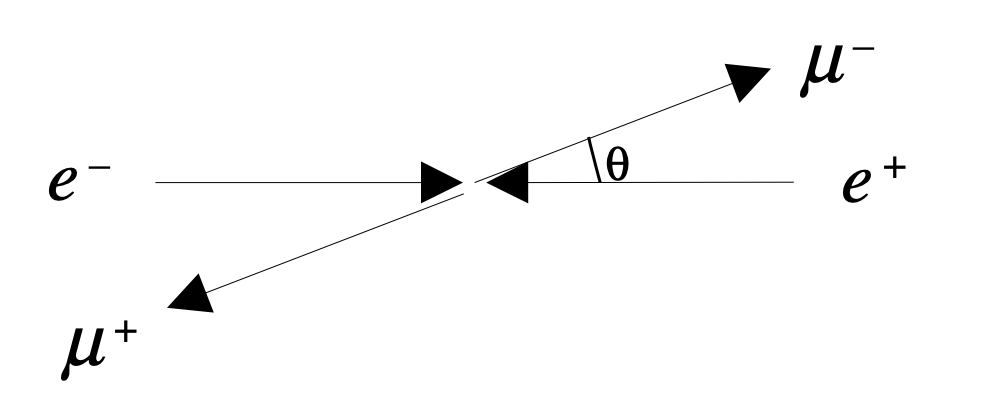
\includegraphics[width=0.6\textwidth]{figures/Hypotest/scatter.png}
    \caption{Scattering process $e^{+}e^{-}\rightarrow \mu^{+}\mu^{-}$, with the angle $\theta$ defined as shown}
    \label{fig:eemm}
\end{figure}
 \begin{figure}
     \centering
     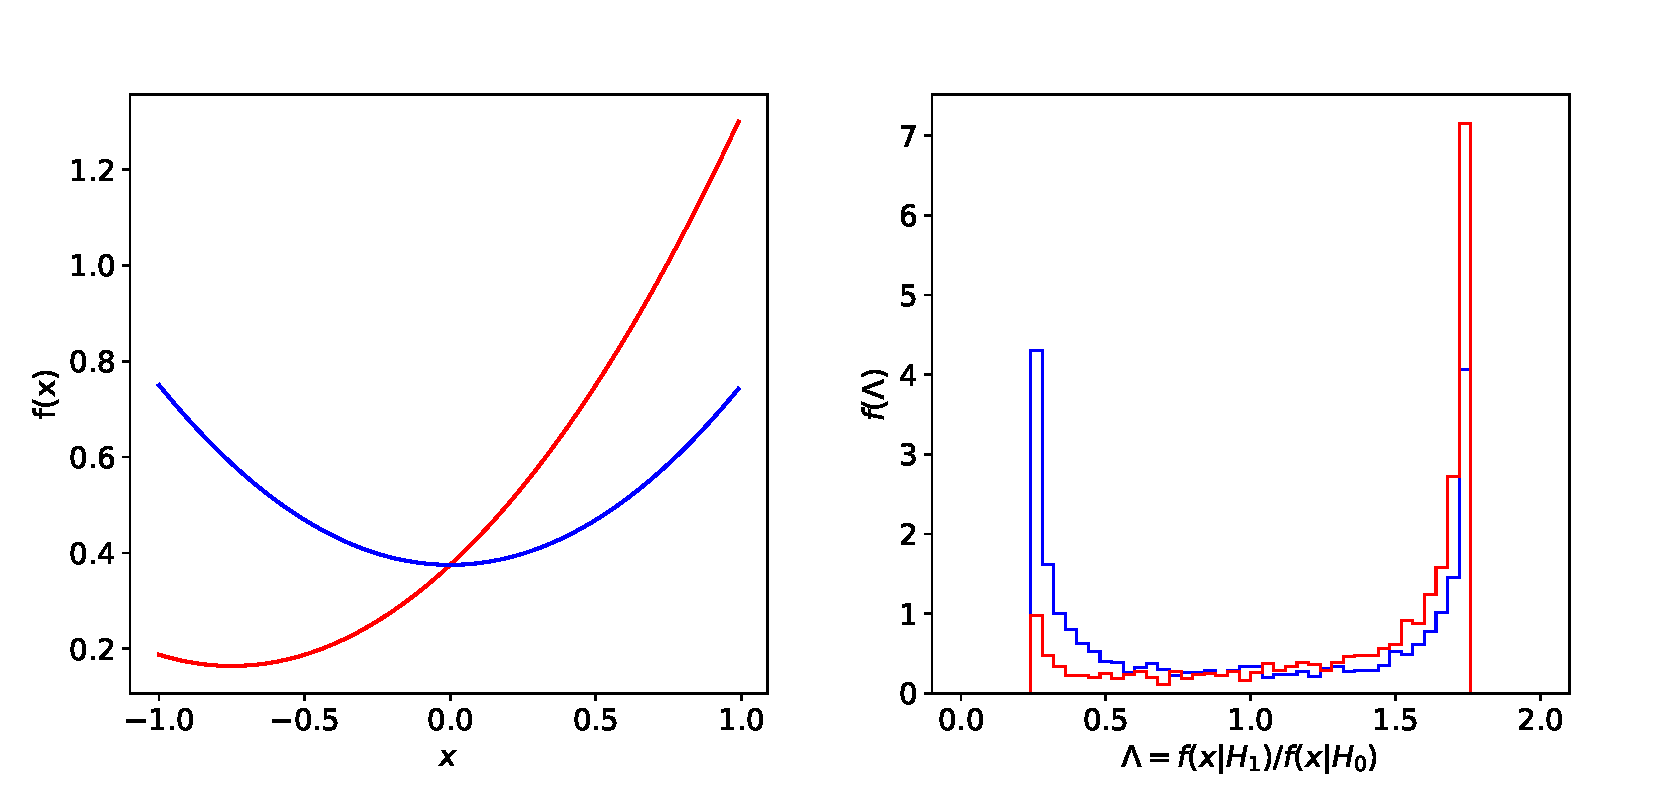
\includegraphics[width=\textwidth]{figures/Hypotest/densities.pdf}
     \caption{Left: probability densities for $x$ under $H_0$ (uniform, blue line) and $H_1$ (cosine, red line). Right: distribution of $\Lambda$ for 5000 pseudo-observations under $H_0$ (blue histogram) and $H_1$ (red histogram).}
     \label{fig:lhclassification}
 \end{figure}
